\documentclass[border=10pt]{standalone}
\usepackage{tikz}
\usetikzlibrary{arrows.meta,calc,decorations.pathmorphing}

\begin{document}
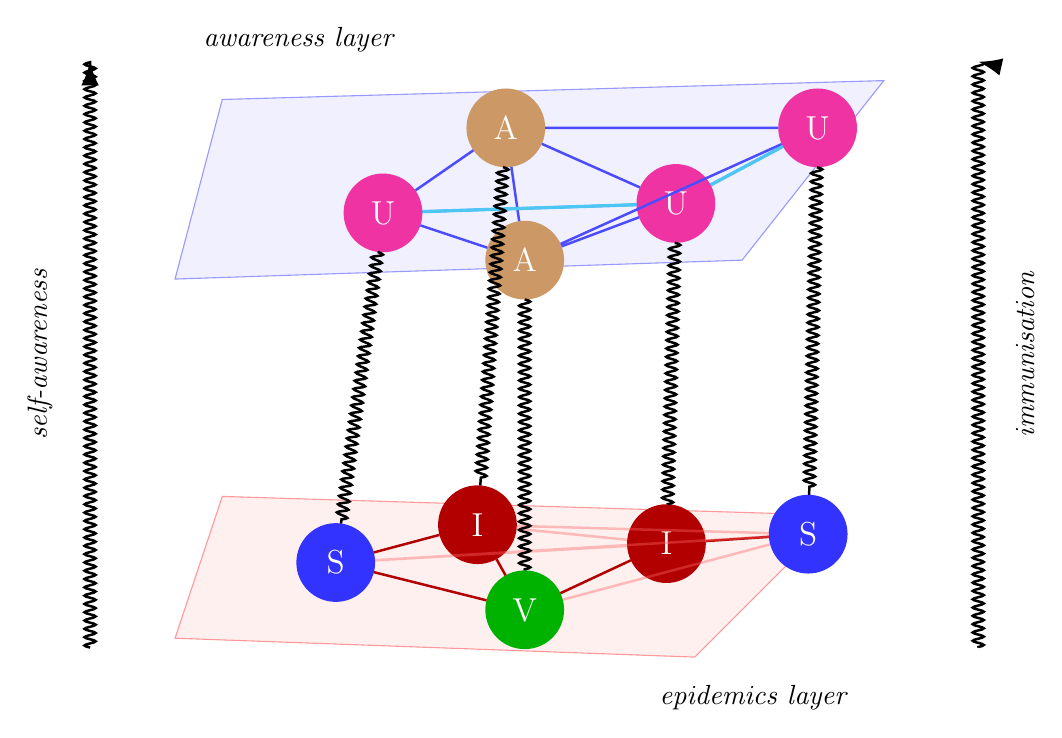
\begin{tikzpicture}[scale=1.2,
    font=\sffamily,
    node distance=2cm,
    >=Latex,
    every node/.style={inner sep=0pt,outer sep=0pt},
    aware/.style={circle,minimum size=10mm,draw=none,fill=brown!80,text=white,font=\large},
    unaware/.style={circle,minimum size=10mm,draw=none,fill=magenta!80,text=white,font=\large},
    sus/.style={circle,minimum size=10mm,draw=none,fill=blue!80,text=white,font=\large},
    inf/.style={circle,minimum size=10mm,draw=none,fill=red!70!black,text=white,font=\large},
    vac/.style={circle,minimum size=10mm,draw=none,fill=green!70!black,text=white,font=\large},
    wavylink/.style={decorate,decoration={coil,aspect=0,segment length=3pt,amplitude=2pt}}
]

% Coordinates for planes (in a simple perspective)
% bottom (epidemics) layer corners
\coordinate (E1) at (-3,-3);
\coordinate (E2) at (3.5,-3.2);
\coordinate (E3) at (2,-4.7);
\coordinate (E4) at (-3.5,-4.5);

% top (awareness) layer corners
\coordinate (A1) at (-3,1.2);
\coordinate (A2) at (4,1.4);
\coordinate (A3) at (2.5,-0.5);
\coordinate (A4) at (-3.5,-0.7);

% Draw planes
\fill[blue!20,opacity=0.3] (A1)--(A2)--(A3)--(A4)--cycle;
\draw[blue!40] (A1)--(A2)--(A3)--(A4)--cycle;

\fill[red!20,opacity=0.3] (E1)--(E2)--(E3)--(E4)--cycle;
\draw[red!40] (E1)--(E2)--(E3)--(E4)--cycle;

% Awareness nodes (top layer)
\node[unaware] (U1) at (-1.3,0.0) {U};
\node[aware]   (A5) at (0.0,0.9) {A};
\node[aware]   (A6) at (0.2,-0.5) {A};
\node[unaware] (U2) at (1.8,0.1) {U};
\node[unaware] (U3) at (3.3,0.9) {U};

% Epidemics nodes (bottom layer)
\node[sus] (S1) at (-1.8,-3.7) {S};
\node[inf] (I1) at (-0.3,-3.3) {I};
\node[vac] (V1) at (0.2,-4.2) {V};
\node[inf] (I2) at (1.7,-3.5) {I};
\node[sus] (S2) at (3.2,-3.4) {S};

% Edges on awareness layer
\draw[blue!70,line width=0.9pt] (U1)--(A5) (U1)--(A6) (U1)--(U2);
\draw[blue!70,line width=0.9pt] (A5)--(A6) (A5)--(U2) (A5)--(U3) (A6)--(U2) (A6)--(U3) (U2)--(U3);
\draw[cyan!70,line width=1.2pt] (U1)--(U2) (U2)--(U3);

% Edges on epidemics layer
\draw[red!70!black,line width=0.9pt]
   (S1)--(I1) (S1)--(V1) (I1)--(V1) (V1)--(I2) (I2)--(S2);
\draw[red!60,opacity=0.4,line width=0.9pt]
   (S1)--(I2) (S1)--(S2) (I1)--(I2) (I1)--(S2) (V1)--(S2);

% Vertical wavy links between layers
\draw[black,line width=0.9pt,wavylink] (U1) -- (S1);
\draw[black,line width=0.9pt,wavylink] (A5) -- (I1);
\draw[black,line width=0.9pt,wavylink] (A6) -- (V1);
\draw[black,line width=0.9pt,wavylink] (U2) -- (I2);
\draw[black,line width=0.9pt,wavylink] (U3) -- (S2);

% Side wavy arrows
\draw[black,line width=0.9pt,wavylink,-{Latex[length=3mm]}] (-4.4,-4.6) -- (-4.4,1.6);
\draw[black,line width=0.9pt,wavylink,{Latex[length=3mm]}-] (5.0,1.6) -- (5.0,-4.6);

% Labels on sides
\node[anchor=south,rotate=90,font=\itshape] at (-4.8,-1.5) {self-awareness};
\node[anchor=north,rotate=90,font=\itshape] at (5.4,-1.5) {immunisation};

% Layer labels
\node[anchor=south west,font=\itshape] at (-3.2,1.7) {awareness layer};
\node[anchor=north east,font=\itshape] at (3.6,-5.0) {epidemics layer};

\end{tikzpicture}
\end{document}